\begin{FlowRevisionText}
\par\medskip
\noindent\textbf{افزایش تطبیقی ذرات با رهاسازی‌های متنوع.}\par\smallskip
مطالعه‌ای مستقل برای نه پروفایل ورودی انجام شد.
نتایج این مطالعه به مقایسهٔ پیشین افزوده شده‌اند.
مکان، تندی و جهت رهاسازی ذرات افزوده متنوع بودند.
بخشی از شرایط رهاسازی با بذر تصادفی ثابت انتخاب شدند.
سرعت اولیه و موقعیت اولیهٔ هر ذره معلوم بودند.
مسیرها رهاسازی‌های مستقل در جریان یکسان را نمایندگی می‌کنند.
برهم‌کنش ذرات در این مدل لحاظ نشده است.
مسیرهای مرجع از میدان اجزای محدود ذخیره‌شده تولید شدند.
در هر مرحله، مسیرهای مرحلهٔ قبل حفظ شدند.
نویز هر مسیر نیز میان مراحل یکسان ماند.

تعداد ذرات با توجه به خطای پروفایل افزایش یافت.
سپس حدود شش مرحلهٔ میانی واقعاً برازش شدند.
منحنی‌های میانی، درون‌یابی پاسخ‌های ابتدا و انتها نیستند.
حد ارزیابی خطای پروفایل $5\%$ و سقف تعداد ذرات $24$ بود.
توقف ناشی از سکون خطا نیز جداگانه ثبت شد.
حقیقت ورودی فقط در تولید داده و ارزیابی استفاده شد.
انتخاب تعداد بر پایهٔ حقیقت، مخصوص همین آزمایش مصنوعی است.
این قاعده، بدون حقیقت معلوم، معیار توقف دادهٔ واقعی نیست.
وزن‌های شبکهٔ مستقیم در تمام برازش‌ها ثابت ماندند.
هر شروع بهینه‌سازی حداکثر $200$ تکرار داشت.
دو شروع در هر برازش بررسی شدند.
در برازش‌های تازه، پاسخ مرحلهٔ قبلی نیز نقطهٔ شروع بود.
همگرایی بهینه‌ساز با رسیدن به خطای کوچک یکسان نیست.

شکل~\ref{fig:adaptive-count-beta5} روند بازسازی ورودی بتای باریک را نشان می‌دهد.
خطای پروفایل در مرحلهٔ $6$ذره‌ای برابر $3.09\%$ بود.
\begin{figure}[htbp]
\centering
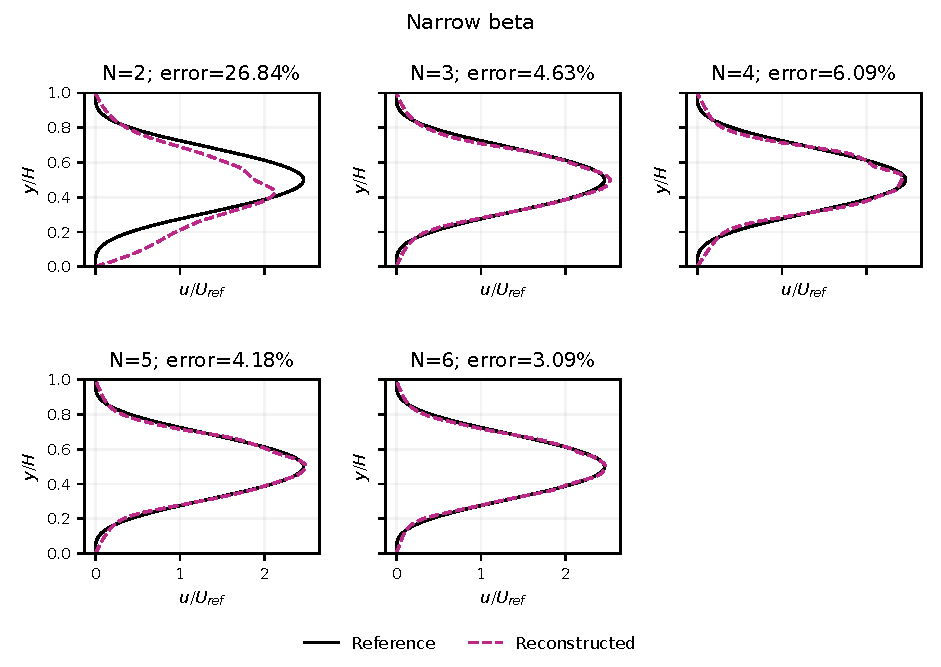
\includegraphics[width=\textwidth]{New_Adaptive_Particle_Results/continuation/figures/beta5.pdf}
\caption[روند بازسازی ورودی بتای باریک با افزایش تطبیقی تعداد ذرات.]{\FlowRevision{روند بازسازی ورودی بتای باریک با افزایش تطبیقی تعداد ذرات.}}
\label{fig:adaptive-count-beta5}
\end{figure}
\FloatBarrier
شکل~\ref{fig:adaptive-count-skew_b3} روند بازسازی ورودی نامتقارن را نشان می‌دهد.
خطای پروفایل در مرحلهٔ $24$ذره‌ای برابر $4.77\%$ بود.
\begin{figure}[htbp]
\centering
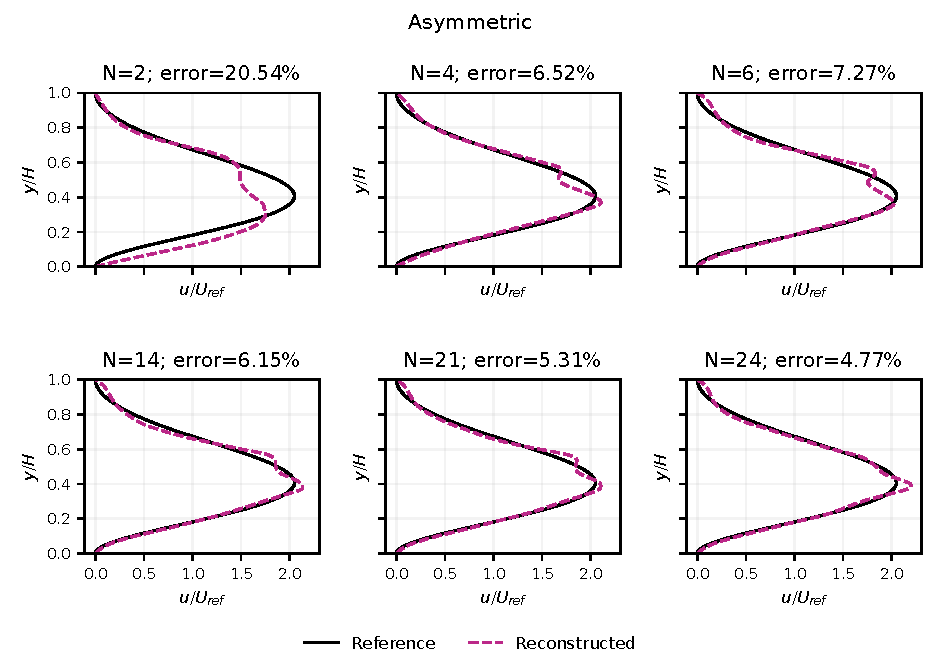
\includegraphics[width=\textwidth]{New_Adaptive_Particle_Results/continuation/figures/skew_b3.pdf}
\caption[روند بازسازی ورودی نامتقارن با افزایش تطبیقی تعداد ذرات.]{\FlowRevision{روند بازسازی ورودی نامتقارن با افزایش تطبیقی تعداد ذرات.}}
\label{fig:adaptive-count-skew_b3}
\end{figure}
\FloatBarrier
شکل~\ref{fig:adaptive-count-flat30} روند بازسازی ورودی تقریباً تخت را نشان می‌دهد.
خطای پروفایل در مرحلهٔ $24$ذره‌ای برابر $6.16\%$ بود.
این نمونه به حد ارزیابی پنج درصد نرسید.
\begin{figure}[htbp]
\centering
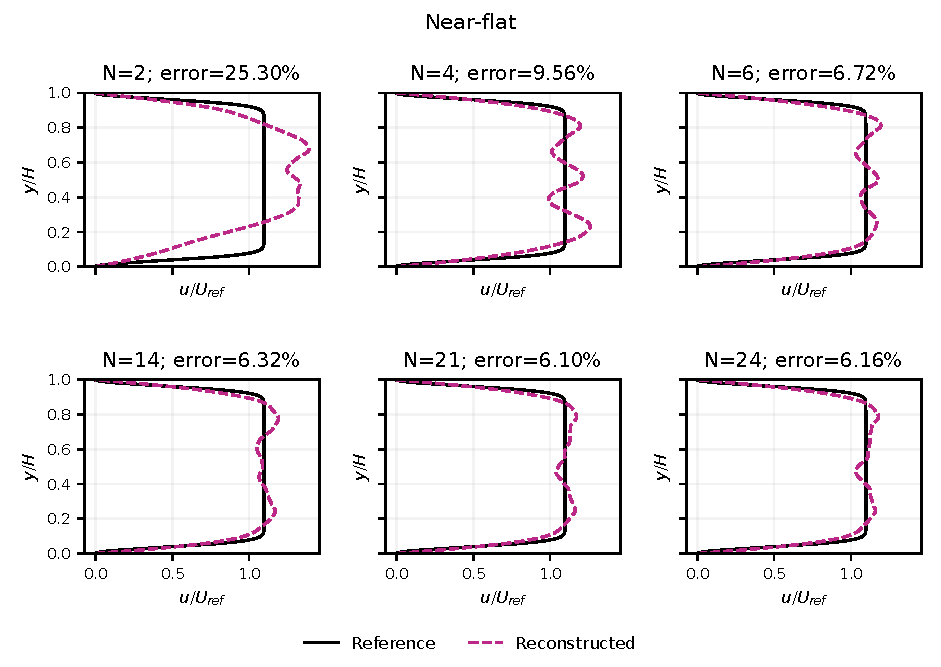
\includegraphics[width=\textwidth]{New_Adaptive_Particle_Results/continuation/figures/flat30.pdf}
\caption[روند بازسازی ورودی تقریباً تخت با افزایش تطبیقی تعداد ذرات.]{\FlowRevision{روند بازسازی ورودی تقریباً تخت با افزایش تطبیقی تعداد ذرات.}}
\label{fig:adaptive-count-flat30}
\end{figure}
\FloatBarrier
شکل~\ref{fig:adaptive-count-twin_b3_r30} روند بازسازی ورودی دوقله‌ای را نشان می‌دهد.
خطای پروفایل در مرحلهٔ $6$ذره‌ای برابر $4.03\%$ بود.
\begin{figure}[htbp]
\centering
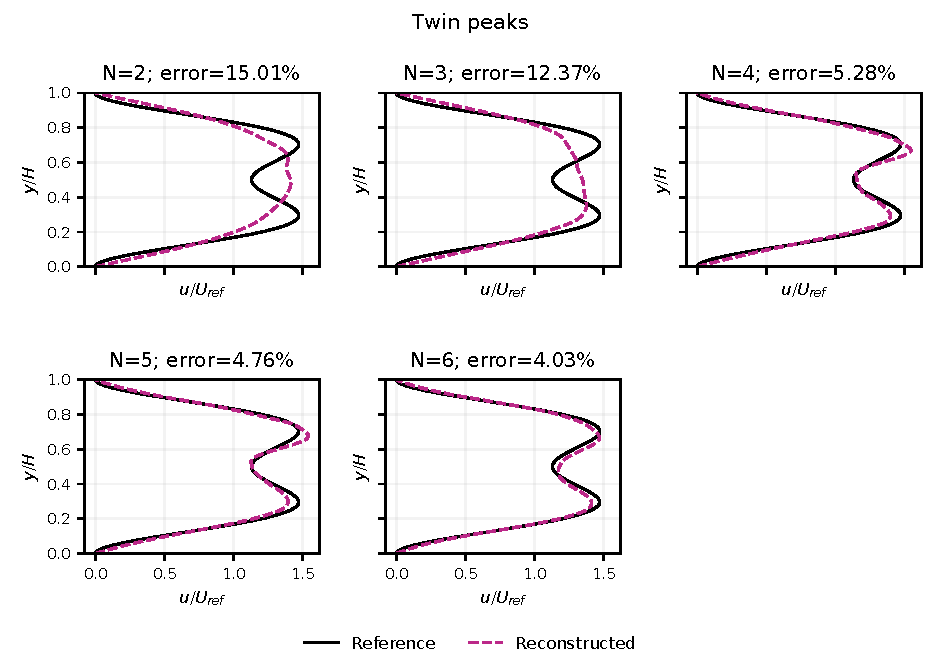
\includegraphics[width=\textwidth]{New_Adaptive_Particle_Results/continuation/figures/twin_b3_r30.pdf}
\caption[روند بازسازی ورودی دوقله‌ای با افزایش تطبیقی تعداد ذرات.]{\FlowRevision{روند بازسازی ورودی دوقله‌ای با افزایش تطبیقی تعداد ذرات.}}
\label{fig:adaptive-count-twin_b3_r30}
\end{figure}
\FloatBarrier
شکل~\ref{fig:adaptive-count-shoulder} روند بازسازی ورودی شانه‌دار را نشان می‌دهد.
خطای پروفایل در مرحلهٔ $24$ذره‌ای برابر $7.88\%$ بود.
این نمونه به حد ارزیابی پنج درصد نرسید.
\begin{figure}[htbp]
\centering
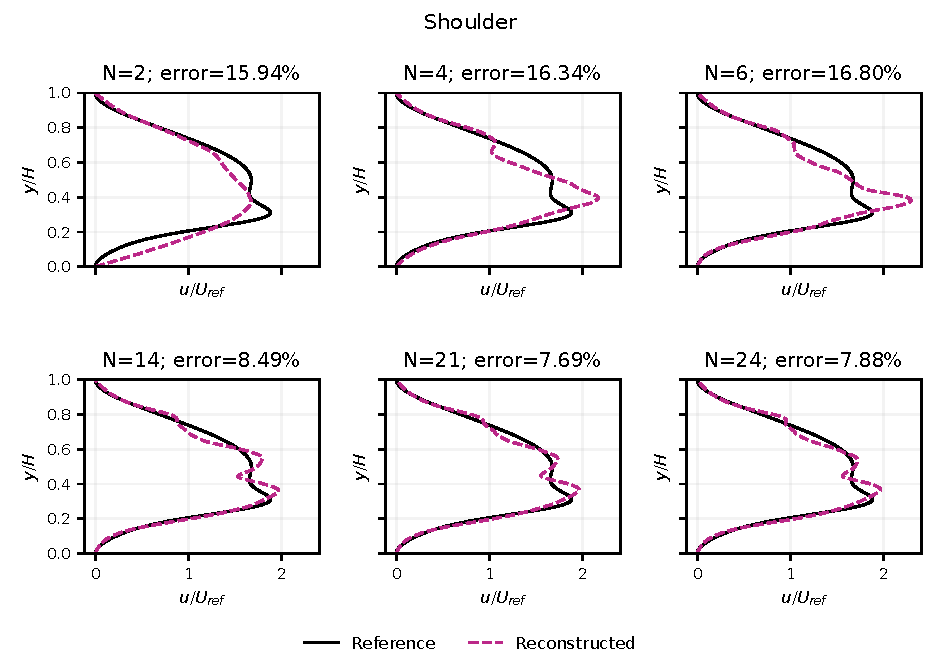
\includegraphics[width=\textwidth]{New_Adaptive_Particle_Results/continuation/figures/shoulder.pdf}
\caption[روند بازسازی ورودی شانه‌دار با افزایش تطبیقی تعداد ذرات.]{\FlowRevision{روند بازسازی ورودی شانه‌دار با افزایش تطبیقی تعداد ذرات.}}
\label{fig:adaptive-count-shoulder}
\end{figure}
\FloatBarrier
شکل~\ref{fig:adaptive-count-mixed} روند بازسازی ورودی چندمقیاسی را نشان می‌دهد.
خطای پروفایل در مرحلهٔ $24$ذره‌ای برابر $7.54\%$ بود.
این نمونه به حد ارزیابی پنج درصد نرسید.
\begin{figure}[htbp]
\centering
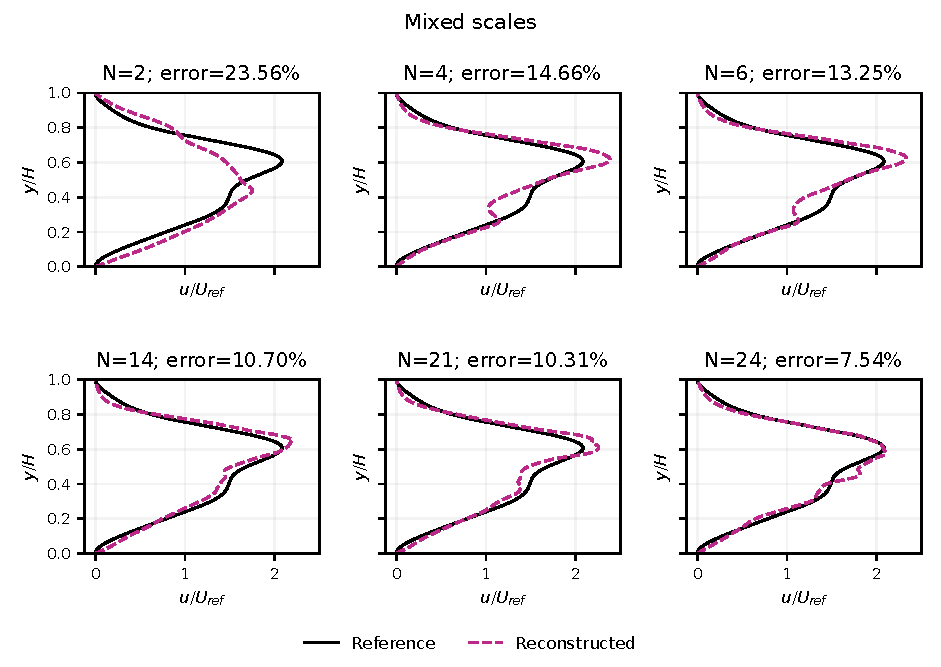
\includegraphics[width=\textwidth]{New_Adaptive_Particle_Results/continuation/figures/mixed.pdf}
\caption[روند بازسازی ورودی چندمقیاسی با افزایش تطبیقی تعداد ذرات.]{\FlowRevision{روند بازسازی ورودی چندمقیاسی با افزایش تطبیقی تعداد ذرات.}}
\label{fig:adaptive-count-mixed}
\end{figure}
\FloatBarrier
شکل~\ref{fig:adaptive-count-waves3_r30} روند بازسازی ورودی سه‌نوسانی را نشان می‌دهد.
خطای پروفایل در مرحلهٔ $24$ذره‌ای برابر $6.87\%$ بود.
این نمونه به حد ارزیابی پنج درصد نرسید.
\begin{figure}[htbp]
\centering
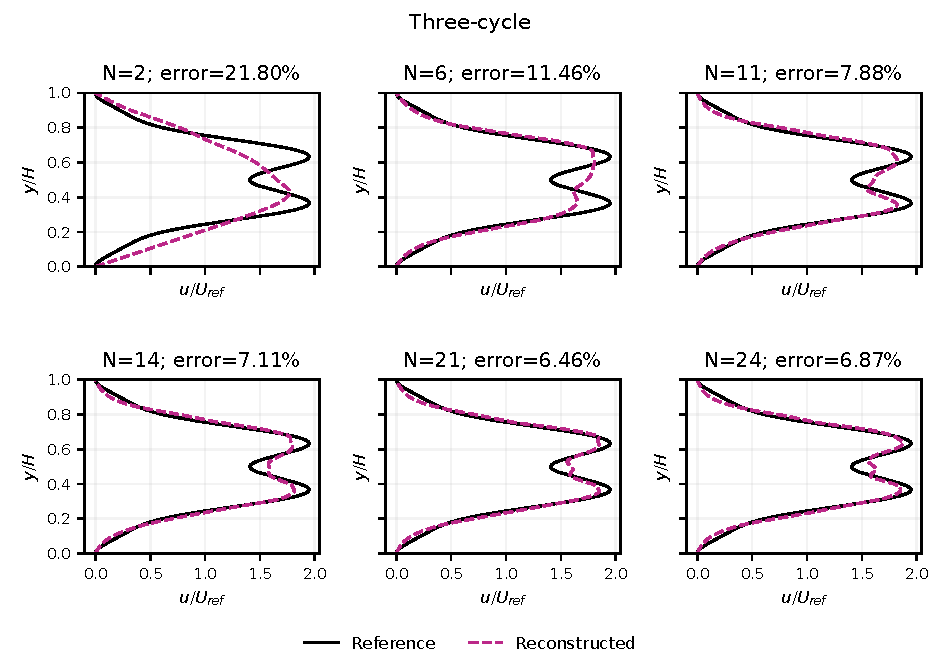
\includegraphics[width=\textwidth]{New_Adaptive_Particle_Results/continuation/figures/waves3_r30.pdf}
\caption[روند بازسازی ورودی سه‌نوسانی با افزایش تطبیقی تعداد ذرات.]{\FlowRevision{روند بازسازی ورودی سه‌نوسانی با افزایش تطبیقی تعداد ذرات.}}
\label{fig:adaptive-count-waves3_r30}
\end{figure}
\FloatBarrier
شکل~\ref{fig:adaptive-count-lobes4_r30} روند بازسازی ورودی چهارنوسانی را نشان می‌دهد.
خطای پروفایل در مرحلهٔ $24$ذره‌ای برابر $18.29\%$ بود.
این نمونه به حد ارزیابی پنج درصد نرسید.
\begin{figure}[htbp]
\centering
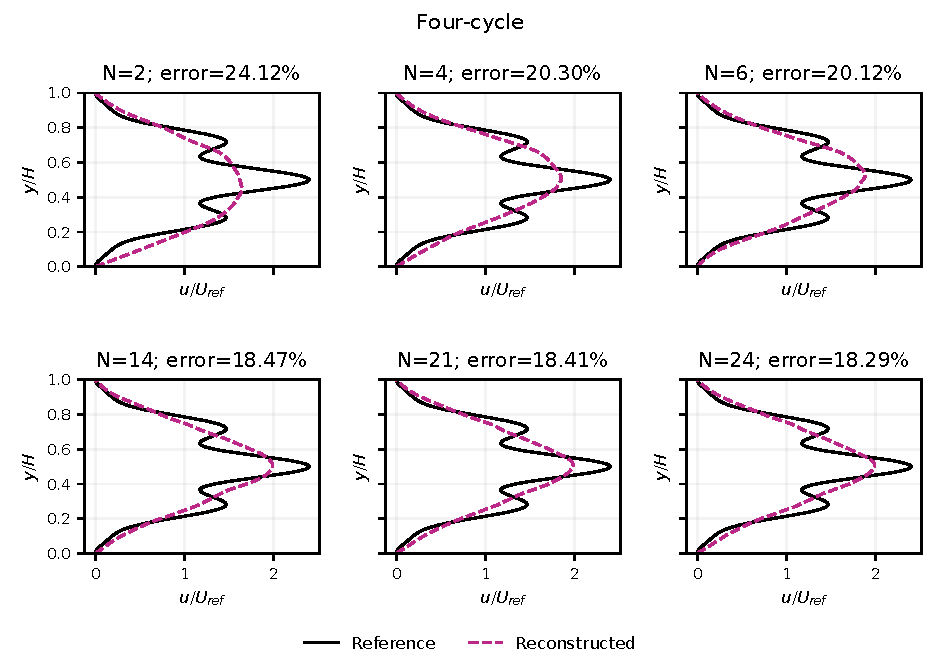
\includegraphics[width=\textwidth]{New_Adaptive_Particle_Results/continuation/figures/lobes4_r30.pdf}
\caption[روند بازسازی ورودی چهارنوسانی با افزایش تطبیقی تعداد ذرات.]{\FlowRevision{روند بازسازی ورودی چهارنوسانی با افزایش تطبیقی تعداد ذرات.}}
\label{fig:adaptive-count-lobes4_r30}
\end{figure}
\FloatBarrier
شکل~\ref{fig:adaptive-count-nine30} روند بازسازی ورودی نه‌نوسانی را نشان می‌دهد.
خطای پروفایل در مرحلهٔ $15$ذره‌ای برابر $38.81\%$ بود.
این نمونه به حد ارزیابی پنج درصد نرسید.
\begin{figure}[htbp]
\centering
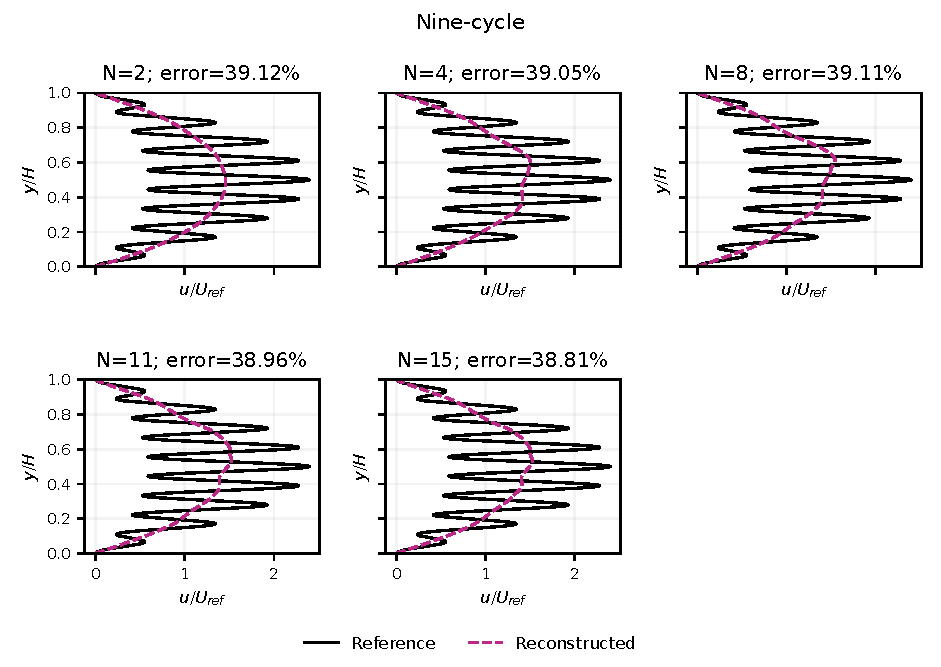
\includegraphics[width=\textwidth]{New_Adaptive_Particle_Results/continuation/figures/nine30.pdf}
\caption[روند بازسازی ورودی نه‌نوسانی با افزایش تطبیقی تعداد ذرات.]{\FlowRevision{روند بازسازی ورودی نه‌نوسانی با افزایش تطبیقی تعداد ذرات.}}
\label{fig:adaptive-count-nine30}
\end{figure}
\FloatBarrier
خطای نهایی به پوشش مسیر، منظم‌سازی و بودجهٔ برازش وابسته است.
از این پیمایش، کمینهٔ قطعی تعداد ذرات نتیجه نمی‌شود.
تعداد پایانی جست‌وجو، الزاماً کمترین تعداد موفقِ ارزیابی‌شده نیست.
\FloatBarrier
\par\medskip
\noindent\textbf{طراحی هدفمند برای نمونهٔ دشوار.}\par\smallskip
ذرات افزوده نزدیک ورودی و در ارتفاع‌های مختلف رها شدند.
سرعت‌های اولیه کوچک‌تر و زمان‌های آغاز حرکت متراکم‌تر بودند.
ضریب جریمهٔ زبری به $10^{-8}$ کاهش یافت.
جریمهٔ باقیماندهٔ شبکه در این آزمون اعمال نشد.
وزن‌های شبکه ثابت ماندند و بازپخش مستقل همچنان انجام شد.
سقف تکرار هر شروع در این آزمون $400$ بود.
این آزمون چند عامل را هم‌زمان تغییر می‌دهد.
اثر جداگانهٔ این عوامل از این مقایسه نتیجه نمی‌شود.
تنظیمات این آزمون، انتخاب اکتشافیِ همین مطالعهٔ مصنوعی هستند.
پاسخ پایه فقط در تعدادهای مشترک برای مقایسه رسم شد.
شکل~\ref{fig:adaptive-near-nine30} مراحل این طراحی تکمیلی را نشان می‌دهد.
خطای پروفایل در مرحلهٔ $24$ذره‌ای برابر $10.59\%$ بود.
\begin{figure}[htbp]
\centering
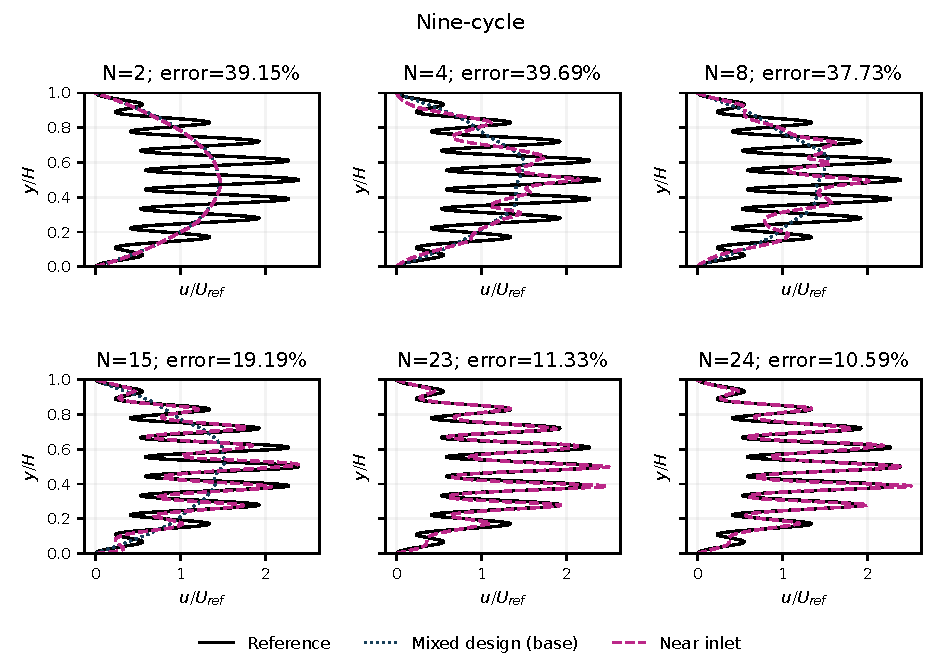
\includegraphics[width=\textwidth]{New_Adaptive_Particle_Results/near_inlet/figures/nine30.pdf}
\caption[روند بازسازی نمونهٔ دشوار با رهاسازی هدفمند نزدیک ورودی.]{\FlowRevision{روند بازسازی نمونهٔ دشوار با رهاسازی هدفمند نزدیک ورودی.}}
\label{fig:adaptive-near-nine30}
\end{figure}
\FloatBarrier
\end{FlowRevisionText}
